\epi{``对此感兴趣,并且希望做点什么。''}
{\textit{在为~Go 添加复数支持时}\\ \textsc{KEN THOMPSON}}

\noindent{}什么是~Go?来自其网站\cite{go_web}的介绍:
\begin{quote}
Go 编程语言是一个使得程序员更加有效率的开源项目。Go 是有表达力、简洁、清晰和有效率的。
它的并行机制使其很容易编写多核和网络应用,而新奇的类型系统允许构建有弹性的模块化程序。
Go 编译到机器码非常快速,同时具有便利的垃圾回收和强大的运行时反射。
它是快速的、静态类型编译语言,但是感觉上是动态类型的,解释型语言。
\end{quote}

Go 1 是~Go 语言的第一个稳定发布版本。
本文档的所有练习都工作于~Go 1 -- 如果不行,那就是~bug。

本书使用了下面的约定:
\begin{itemize}
\item 代码用~\prog{楷体} 显示;
\item 关键词用~\key{楷体粗体} 显示;
\item 注释用~\rem{楷体斜体} 显示;
\item 代码中额外的标记,\coderemark{用这种形式展现};
\item 使用数字~\gocircle{1} 标记长内容 -- 解释会跟随其后;
\item 行号在右边展示;
\item Shell 示例用~\pr{} 作为标记;
\item 强调的段落会缩进,在左边有竖线。
\end{itemize}

\section{官方文档}
Go 已经有大量的文档。
\gomarginpar{在互联网上搜索时,应当使用``golang''这个词来代替原始的``go''。}
例如~Go Tutorial \cite{go_tutorial} 和~Effective Go \cite{effective_go}。
网站~\url{http://golang.org/doc/} 也是绝佳的起点 
\footnote{\url{http://golang.org/doc/} 本身是由~Go 程序~\prog{godoc} 提供服务的。}。
虽然并不一定要阅读这些文档,但是强烈建议这么做。

Go 1 可以用两个程序提供文档服务:
\begin{enumerate}
\item \prog{go doc},该程序用于(第三方)\emph{包}文档;
\item \prog{godoc},用于官方包文档,例如~Go 1 相关的所有内容。
\end{enumerate}

这两个最明显的区别在于内建文档(参阅下一章的``\titleref{sec:builtins}``):
\begin{display}
\pr \user{go doc builtin}   \coderemark{35 lines}
\pr \user{godoc builtin}    \coderemark{242 lines}
\end{display}

通常这两个的区别并无大碍,不过要留意~\prog{go doc} 和~\prog{godoc} 并不等同。
在第~\ref{chap:packages} 章解释了如何构造你自己的包的文档。

\section{前身}
Go 的前身来自于~Inferno\cite{inferno}(基于~Plan 9\cite{plan9} 的改造)。
Inferno 包含了一个叫做~Limbo\cite{limbo} 的语言。这里引用了一段来自于~Limbo 论文的描述:
\begin{quote}
Limbo 是用于开发运行在小型计算机上的分布式应用的编程语言。
它支持模块化编程,编译期和运行时的强类型检查,\emph{进程内基于具有类型的~channel 通讯},
原子性\emph{垃圾收集},和简单的抽象数据类型。
它被设计用于即便是没有硬件内存保护的小型设备上,也能安全的运行。
\end{quote}
Go 从~Limbo 继承的另一个特性是~channel(参阅第~\ref{chap:channels} 章)。
从~Limbo 文档来的另一段描述:
\begin{quote}
[channel] 是用于向系统中其他代理发送和接收特定类型对象的通讯机制。
channel 可以用于本地进程间通讯;用于连接到命名的目的地的库方法。
两种情况都是直接发送和接收操作的。
\end{quote}
在~Go 中,channel 比在~Limbo 中更加好用。
如果我们对~Go 的历史深入探索,会发现一个到~``Newsqueak''\cite{newsqueak} 的引用,
这是在类~C 语言中使用~channel 通讯的拓荒者。
channel 对于这些语言并不是独一无二的,另一个非类~C 语言,Erlang\cite{erlang},也在使用它。

\begin{figure}[H]
\caption{Go 编年史}
\label{fig:chrono-of-go}
\begin{center}
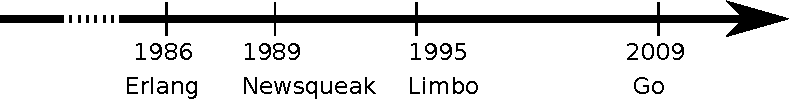
\includegraphics[scale=0.65]{fig/go-history.pdf}
\end{center}
\end{figure}

使用~channel 与其他进程进行通讯的办法,
叫做通讯序列化过程(Communicating Sequential Processes - CSP),
由~C. A. R. Hoare\cite{hoare} 设计构想,而他正是那个发明快速排序\cite{quicksort}算法的人。

\begin{lbar}[]
Go 是第一个实现了简单的(或更加简单的)并行开发的、跨平台类~C 语言。
\end{lbar}

\section{获得 Go}
在这一节中将介绍如何在本地设备上安装~Go,不过也可以在线上 \url{http://play.golang.org/} 编译~Go 代码。这是最为便捷的尝试方法。

也可以从网站\cite{go_install}获得已经编译好的二进制版本。

Ubuntu 和~Debian 在其仓库中都有~Go 包,可以查找``golang''包。
但是工作的时候会有一些小问题。所以现在仍然使用源码进行安装。

手工从~mercurial 中获取~Go 代码并且编译。对于其他类~Unix 系统,过程类似。
\begin{itemize}
\item 首先安装~Mercurial(获取~\prog{hg} 命令)。
在~Ubuntu/Debian/Fedora 需要安装~\prog{mercurial} 包;

\item 为了编译~Go 需要包:\prog{bison},\prog{gcc},\prog{libc6-dev},\prog{ed},\prog{gawk} 和\prog{make};

\item 设置环境变量~\prog{GOROOT} 作为~Go 的安装目录:
\begin{display}
\pr \user{export GOROOT=\~{}/go}
\end{display}

\item 然后获取~Go 最新的发布版(=Go 1)源代码:
\begin{display}
\pr \user{hg clone -r release https://go.googlecode.com/hg/ \$GOROOT}
\end{display}

\item 设置~PATH 指向到~Go 的二进制文件所在目录,这样就可以让~Shell 找到它们:
\begin{display}
\pr \user{export PATH=$GOROOT/bin:$PATH}
\end{display}

\item 编译~Go
\begin{display}
\pr \user{cd \$GOROOT/src}
\pr \user{./all.bash}
\end{display}
\end{itemize}
如果全部都没问题,你最终会看到下面的内容:
\begin{display}
+--- cd ../test
+0 known bugs; 0 unexpected bugs
+
+ALL TESTS PASSED
+
+---
+Installed Go for linux/amd64 in /home/go
+Installed commands in /home/go/bin
\end{display}

\section{在~Windows 下获得~Go}

最好的方式是遵从网站\cite{go_install}的介绍,为了方便重复如下。

\begin{itemize}
\item 下载~Go-1:
\url{http://code.google.com/p/go/downloads/list?q=OpSys-Windows+Type%3DArchive};
\item 解压缩到~\verb|C:\| 盘;
\item 确保内容在~\verb|C:\Go|。注意:在解压缩~zip 文件时,这个目录会被创建;
\item 添加~\verb|C:\Go\bin| 到~\$PATH:
\begin{display}
export PATH=\verb|C:\Go\bin|
\end{display}
\end{itemize}

\section{练习}
\begin{Exercise}[title={文档},difficulty=1]
\label{ex:doc}
\Question
Go 的文档可以通过~\prog{go doc} 程序阅读,它包含在~Go 的发布包中。

\prog{go doc hash} 给出了~\package{hash} 包的信息:
\vskip\baselineskip
\begin{display}
\pr \user{go doc hash}
PACKAGE

package hash

...
...
...

SUBDIRECTORIES

        adler32
        crc32
        crc64
        fnv

\end{display}
\vskip\baselineskip
哪个~\prog{go doc} 的命令可以显示~\package{hash} 包中的~\package{fnv} 文档?

\end{Exercise}

\begin{Answer}
\Question
\package{fnv} 包在~\package{hash} 的\emph{子目录}中,所以只需要 
\quad \texttt{go doc hash/fnv} 即可。


所有的内建函数同样可以通过~\prog{godoc} 程序访问:\prog{go doc builtin}。
\end{Answer}


\cleardoublepage
\section{答案}
\shipoutAnswer
